\documentclass[9pt]{beamer}

\beamertemplatenavigationsymbolsempty
\renewcommand\mathfamilydefault{cmr}

\usepackage{pajmath}
\usepackage{booktabs}
\usepackage{colortbl}

\usepackage{tikz}
\usetikzlibrary{positioning,shapes.misc,calc,backgrounds,scopes} 
\usetikzlibrary{datavisualization}
\usetikzlibrary{datavisualization.formats.functions}
\tikzset{boxed/.style={
  thick,
  draw=black,
  top color=white,
  text height=1.5ex,
  text depth=.25ex
}}


\newcommand\lo{$-1$}
\newcommand\hi{$\phan1$}
\newcommand\ze{$\phan0$}
\newcommand\Ze{$\phan\Vzero$}
\newcommand\pskip{\pause\bigskip}
\newcommand\lspace{\addtolength{\itemsep}{0.5\baselineskip}}
\newcommand\red[1]{{\color{red}#1}}

\title{Reinforcement Learning:\\Value Functions}
\author{BIOE 498/598 PJ}
\date{Spring 2021}

\begin{document}
\frame{\titlepage}

\begin{frame}{Review}

\textbf{Last time}
\begin{itemize}\lspace
	\item RL agents learn by trial and error.
	\item RL problems are formulated as MDPs.
	\item Monte Carlo methods can find policies for RL problems.
	\item<2-> \textbf{Today:} What exactly is Monte Carlo learning?
\end{itemize}
	
\end{frame}

\begin{frame}{A Monte Carlo approach for Gridworld}

\begin{columns}
\begin{column}{0.5\textwidth}
	\begin{itemize}
		\item Each grid square is a state.
		\item Actions: move up, down, left, or right, but the agent cannot leave the grid.
		\item Reward: $-1$ for each step.
		\item Policy: Random.
	\end{itemize}
	
\bigskip
Starting from a random state, make random moves until the agent reaches the end.

\bigskip
Repeat may times and average the total rewards from each trajectory.

\bigskip
The policy is to move to squares with better Monte Carlo returns.
\end{column}

\begin{column}{0.5\textwidth}
	\begin{center}
		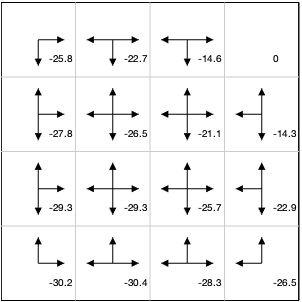
\includegraphics[width=\textwidth]{figures/gridworld1a.png}	
	\end{center}
\end{column}

\end{columns}

\end{frame}

\begin{frame}{Value functions}

\begin{itemize}\lspace
	\item We are using Monte Carlo to learn a \textbf{value function}.
	\item The value of a state is the expected reward from that state to the end of the trajectory.
		\[ V(s_i) = \mathbb{E}\left\{ \sum_{k=i}^T r_k \right\} = \mathbb{E}\{R_i\} \]
	where $R_i$ is the \emph{return} starting at state $s_i$, i.e.\ the cumulative reward for the rest of the trajectory: $R_i = r_i + r_{i+1} + \cdots + r_{T-1} + r_T$.
	\item<2-> If we know the value function we can derive a policy: Take the action that moves to the state with the highest value.
\end{itemize}
	
\end{frame}

\begin{frame}{Trajectories}

\begin{itemize}
	\item A trajectory in an MDP is a sequence of states, actions, and rewards:
		\[ s_0,a_0,r_0,\,s_1,a_1,r_1,\,\ldots,s_{T-1},a_{T-1},r_{T-1},\,s_T,r_T \]
	\item The length $T$ can vary for every trajectory.
	\item There is no action selected in the terminal state $s_T$, but there can be a terminal reward $r_T$.
	\item A reward $r_i$ can be positive (reward), negative (penalty), or zero. Some MDPs only have a nonzero terminal reward!
\end{itemize}
	
\end{frame}

\begin{frame}{From trajectories to value functions}

\begin{columns}
\begin{column}{0.6\textwidth}
Let's calculate $V(s)$ for a $3\times 3$ Gridworld board.

\bigskip
The MDP is deterministic, so knowing $s_i$ and $s_{i+1}$ tells us $a_i$. Also, $r_i=-1$ for all $0\le i<T$.
\end{column}

\begin{column}{0.4\textwidth}
	\begin{center}
		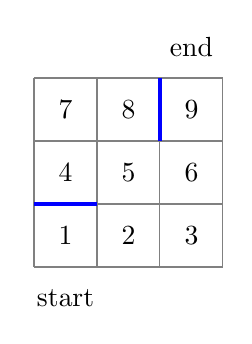
\begin{tikzpicture}[scale=0.8]
			\draw [thin,gray] (0,0) grid (3,3);
			\draw (0.5,0.5) node {1}
				  (1.5,0.5) node {2}
				  (2.5,0.5) node {3}
				  (0.5,1.5) node {4}
				  (1.5,1.5) node {5}
				  (2.5,1.5) node {6}
				  (0.5,2.5) node {7}
				  (1.5,2.5) node {8}
				  (2.5,2.5) node {9};
			\draw (0.5,-0.5) node {start}
				  (2.5,3.5) node {end};
			\draw [very thick,blue] (0,1) -- (1,1) (2,3) -- (2,2);
		\end{tikzpicture}
	\end{center}	
\end{column}
\end{columns}
\pause
\begin{align*}
\tau_1 &:\quad 1,2,5,4,5,6,3,6,9 & R_{\tau_1} &= -8 \\
\tau_2 &:\quad 1,2,3,6,3,2,5,8,7,8,5,6,9 & R_{\tau_2} &= -12 \\
\tau_3 &:\quad 1,2,5,2,3,6,9 & R_{\tau_3} &= -6 \\
\tau_4 &:\quad 1,2,5,4,5,2,3,6,5,8,5,6,3,2,5,6,9 & R_{\tau_4} &= -16 \\
\end{align*}
\pause
\[ V(s_1) \approx \frac{R_{\tau_1} + R_{\tau_2} + R_{\tau_3} + R_{\tau_4}}{4} = \frac{(-8) + (-12) + (-6) + (-16)}{4} = -10.5 \]
	
\end{frame}


\begin{frame}{Re-using our trajectories}

\begin{columns}
\begin{column}{0.6\textwidth}
\begin{align*}
\tau_1 &:\quad 1,\red2,5,4,5,6,3,6,9 \\
\tau_2 &:\quad 1,\red2,3,6,3,\red2,5,8,7,8,5,6,9 \\
\tau_3 &:\quad 1,\red2,5,\red2,3,6,9 \\
\tau_4 &:\quad 1,\red2,5,4,5,\red2,3,6,5,8,5,6,3,\red2,5,6,9 \\
\end{align*}
\end{column}

\begin{column}{0.4\textwidth}
	\begin{center}
		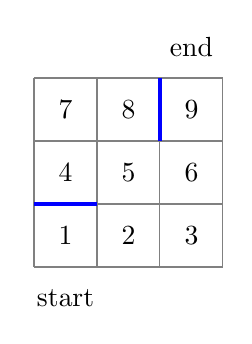
\begin{tikzpicture}[scale=0.8]
			\draw [thin,gray] (0,0) grid (3,3);
			\draw (0.5,0.5) node {1}
				  (1.5,0.5) node {2}
				  (2.5,0.5) node {3}
				  (0.5,1.5) node {4}
				  (1.5,1.5) node {5}
				  (2.5,1.5) node {6}
				  (0.5,2.5) node {7}
				  (1.5,2.5) node {8}
				  (2.5,2.5) node {9};
			\draw (0.5,-0.5) node {start}
				  (2.5,3.5) node {end};
			\draw [very thick,blue] (0,1) -- (1,1) (2,3) -- (2,2);
		\end{tikzpicture}
	\end{center}	
\end{column}
\end{columns}

\pskip
We can estimate $V(s_2)$ using the same trajectories because of the Markov Property. Every visit to $s_2$ is equivalent to new trajectory that begins at $s_2$.

\pskip
Some trajectories visit $s_2$ more than once. For example, $\tau_3$ has two returns $R=-5$ and $R=-3$.

\end{frame}

\begin{frame}{Summary}

\begin{itemize}\lspace
	\item RL agents can learn by trial and error.
	\item MDPs provide a mathematical structure for RL problems.
	\item The choice of states, actions, and rewards is critical.
	\item<2-> \textbf{Next time:} What are we learning from our random maze walks?
\end{itemize}

\end{frame}

\end{document}
